% ---------------------------------------------------------------------------
% Author guideline and sample document for EG publication using LaTeX2e input
% D.Fellner, v1.13, Jul 31, 2008

\documentclass{egpubl-eurovis-short}
\usepackage{eurovis2014-short}

% --- for EuroVis
%\WsSubmission    % uncomment for submission to EuroVis
\WsPaper         % uncomment for final version of EuroVis contribution

\electronicVersion % can be used both for the printed and electronic version

% !! *please* don't change anything above
% !! unless you REALLY know what you are doing
% ------------------------------------------------------------------------

% for including postscript figures
% mind: package option 'draft' will replace PS figure by a filname within a frame
\ifpdf \usepackage[pdftex]{graphicx} \pdfcompresslevel=9
\else \usepackage[dvips]{graphicx} \fi

\PrintedOrElectronic

% prepare for electronic version of your document
\usepackage{t1enc,dfadobe}

\usepackage{egweblnk}
\usepackage{cite}

% For backwards compatibility to old LaTeX type font selection.
% Uncomment if your document adheres to LaTeX2e recommendations.
% \let\rm=\rmfamily    \let\sf=\sffamily    \let\tt=\ttfamily
% \let\it=\itshape     \let\sl=\slshape     \let\sc=\scshape
% \let\bf=\bfseries

% end of prologue

%\input{EGauthorGuidelines-body.inc} % commented by KK for ShareLaTeX use

% ---------------------------------------------------------------------
% EG author guidelines plus sample file for EG publication using LaTeX2e input
% D.Fellner, v1.17, Sep 23, 2010


\title[Transfer function design gallery]%
      {Transfer function design gallery}

% For anonymous conference submission, please enter your SUBMISSION ID.
\author[Klemen Stanič, 63150267]{Klemen Stanič, 63150267}

%% For the final version of your accepted paper, please enter the authors names and affiliations.
%\author[D. Fellner \& S. Behnke]
%       {D.\,W. Fellner\thanks{Chairman Eurographics Publications Board}$^{1,2}$
%        and S. Behnke$^{2}$
%        \\
%         $^1$TU Darmstadt \& Fraunhofer IGD, Germany\\
%         $^2$Institut f{\"u}r ComputerGraphik \& Wissensvisualisierung, TU Graz, Austria
%       }

% ------------------------------------------------------------------------

% if the Editors-in-Chief have given you the data, you may uncomment
% the following five lines and insert it here
%
% \volume{27}   % the volume in which the issue will be published;
% \issue{1}     % the issue number of the publication
% \pStartPage{1}      % set starting page


%-------------------------------------------------------------------------
\begin{document}

% \teaser{
%  
\includegraphics[width=\linewidth]{eg_new}
%  \centering
%   \caption{New EG Logo}
% \label{fig:teaser}
% }

\maketitle

\begin{abstract}
We present the implementation of an exploratory tool, which aids users in the process of transfer function creation, in the context of a 3D volume rendering. The approach uses a combination of 3D volume analysis and a transfer function design gallery. Through iterations, the user is guided to a final transfer function, with visual feedback and ability to adjust the transfer function at every step.
\end{abstract}





%-------------------------------------------------------------------------
\section{Introduction}
Direct volume rendering presents an effective method of arbitrary tomographic data visualization. Apart from medical applications, this process is widely used in engineering, industrial design and many other fields. In order to properly represent the volume in a final rendered image, an effective transfer function must be used. Transfer functions map volume data values to colors and different levels of opacities. A popular transfer function design tool is a two-dimensional (2D) canvas, where the axes represent the feature space of the input data. Using this tool, manual definition of transfer functions is possible, but requires a lot of effort through trial and error approach, especially if the user is not familiar with the data. 

In this seminal work, we present an implementation of a iterative process, which helps the user discover the appropriate transfer function for a given dataset. We use the \textit{VPT} application as a basis for our work, and build the additions on top of it. 

This seminal report is organized as follows. In Section 2, we introduce similar research works on transfer functions. In Section 3, we describe our process of transfer function generation and evaluate it in Section 4. Finally, we conclude the work in Section 5.


\section{Related work}
As previously stated, the basis of our work is the \textit{Volumetric Path Tracing} application, presented by the authors in the article Lesar \textit{et. al.} \cite{lesar2018real}. The application is a web application, designed to work in all modern browsers with \textit{WebGL 2.0} support, including mobile devices. It uses a pipeline-like process, which consists of three stages. First, rays are generated and propagated through the volume. During the second stage, the result of the previous stage is integrated and accumulated into a frame. Lastly, the frame is presented to the user by painting it on a canvas element. The application provides many rendering techniques such as the Single Scattering, Multiple Scattering and the Emission-absorption model. The user can create and modify the transfer function using a 2D canvas widget, where axis represent the feature space of the volume.

Many existing transfer function generation tools and techniques are focused on efficient exploration of the parameter space in order to simplify the transfer function generation process. Shen \textit{et.al} first present the design of a 1D histogram based transfer functions, which they than expand to a 2D histogram based transfer functions \cite{shen2012visualization}. 2D histogram is used, where the first dimension represents the distribution of volume intensity at a given voxel and the second dimension represents the distribution of a gradient at a given voxel, in order to more clearly define the bounderies of different tissues (materials) in the volume. Opacity modulation is then used to provide a better visualization of interior parts of the volume.

Yanling \textit{et.al} present their framework for volume exploration of biological datasets \cite{liu2011quick2insight}. They use the K-Means++ clustering algorithm in order to classify the two-dimensional (2D) histogram, created from the data. Colors and opacity levels are then automatically generated, based on the clusters. This approach gives good results, while also providing the user with a simple and intuitive user interface. 

Maciejewski \textit{et.al} present a similar approach, where a process of non-parametric clustering is added to the classic two-dimensional (2D) histogram in order to ease the transfer functions space exploration \cite{maciejewski2009structuring}. Non-parametric kernel density estimation is used to group voxels with similar features within the 2D histogram. These clusters are then binned and colored based on their estimated density. To better extract the regions, the users can interactively grow or shrink the binned regions. Temporal exploration is also added, allowing users to explore the dataset within a given time period without manually changing the transfer function at each frame.

A more general approach to setting parameters in the field of computer graphics is proposed by Marks \textit{et.al}, in the form of a design gallery \cite{marks1997design}. Multidimensional mapping functions, which are hard to intuitively grasp and navigate, are set using the iterative process, where the user is guided through the process with the help of interactive graphics. The proposed idea is presented on multiple computer graphics problems, namely the selection and placement of lights in the space, the definition of transfer functions for volume rendering and animation applications.

\section{Methods}
In this section, we present our implementation of the iterative process, which guides the user through the transfer function generation. First, we describe the main idea of the procedure. After that, we describe each of the steps of the process. Lastly, we describe the specifics of the gallery image rendering.

\subsection{Main idea}
In order to simplify the process of creating and adjusting the transfer function for good visualization in volume rendering, we add a design gallery widget to the \textit{VPT} application. We separate the process of transfer function definition into three steps. The first step consists of a feature extraction from the dataset. The result is then presented to the user in the second step, in a form of multiple rendered images, where each image was constructed using a different transfer function. The user then selects the rendered image he deems most appropriate, and the associated transfer function is then further refined with subsequent iterations in step 3. During the process, the user can manually adjust the transfer functions at each iteration, while retaining the full control of the renderer, such as the position of the volume on the canvas, zoom, translations and the renderer properties (extinction value, scattering albedo value, the tonemapper properties, \textit{etc.}).

\subsection{Step 1: Feature extraction}
Automatic feature extraction of the input dataset is performed using a one-dimensional (1D) histogram, which is constructed during the volume loading process. The peaks of the histogram represent the regions of interest in the input volume, where each peak can be seen as a separate tissue (material) in the volume. A simple peak searching algorithm is used to find the highest values in the histogram, where the peaks in close proximity of each other are discarded. 

\subsection{Step 2: Identification of irrelevant volume regions}
Top six peaks, obtained in step 1, are each assigned a unique color. Six transfer functions are generated, where each transfer function comprises of 6 vertical lines, whose x-axis placement corresponds to the value of the corresponding peak. The line width is a constant small value (0.05). The line height is also set as a constant, which is set to the maximum value (1.0). Each of the six transfer functions has one color's opacity value set to a lower value of 0.3. The transfer functions are then used to render six distinctive images and are simultaneously presented to the user in a form of a grid gallery. The gallery is presented in the figure \ref{fig:gallery}, the transfer function corresponding to the first gallery item is shown in the figure \ref{fig:tf}. 
This process allows the user to visually identify the irrelevant regions of the volume, such as the material surrounding the scanned object, or the outermost layer of the object, which is obstructing the view of the insides. The user can manually adjust the opacity of the region before continuing to the next step, which is triggered by pressing the \textit{"Iterate gallery button"}, located in the main dialog.


\begin{figure}[htb]
   % an empty figure just consisting of the caption lines
  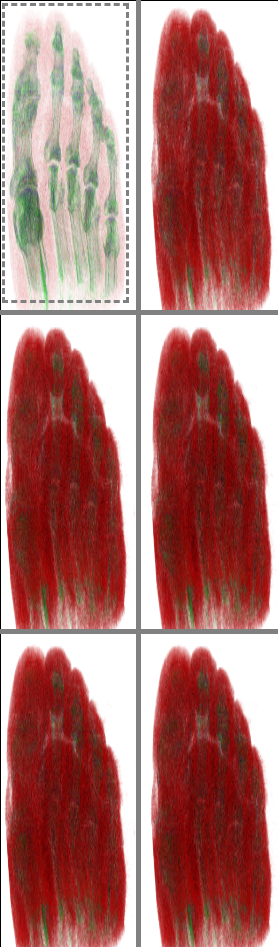
\includegraphics[width=.8\linewidth]{gallery.png}
   \caption{\label{fig:gallery}
     Gallery at step 1: Feature extraction}
\end{figure}

\begin{figure}[htb]
   % an empty figure just consisting of the caption lines
  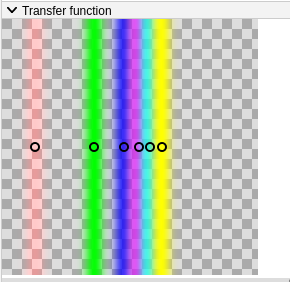
\includegraphics[width=.8\linewidth]{tf.png}
   \caption{\label{fig:tf}
     Transfer function at step 1: Feature extraction}
\end{figure}

\subsection{Step 3: Further refining of the transfer function}
The chosen transfer function is used to generate six new transfer function, the rendering of which are again presented in the gallery. Each of the transfer function has the y-axis position of the first bump (color) in the transfer function shifted by a constant amount, where the height of the bump is also set to a constant value. 
This way, the user is presented with a simultaneous view of all the different renders. 
By changing the y-axis position of the bump in the transfer function, we are trying to locate the position of the bump, where the corresponding region of the volume has the highest gradient. This results in better defined edges between different materials (tissues) in the final rendered image.
This step is iterated for every bump (color) in the transfer function, until all bumps are correctly placed. During the process, the user can manually modify the size, position and opacity of each of the bumps. 

At the end of the whole process, the user is left with a constructed transfer function, which required little to no manual parameter setting and tweaking.
 
\subsection{Gallery image rendering}
Throughout the process of transfer function creation, multiple renders of the volume are presented to the user. A new gallery image is generated every time the user interacts with the scene, changes the renderer or changes any of the render properties, modifies or iterates to a new transfer function \textit{etc}. Each of the gallery items has its own canvas \textit{DOM} element, unto which lower resolution images are rendered by the renderer. To reduce the strain on the hardware resources, image rendering process of each gallery item is stopped, when the quality of the image is sufficient. To accomplish this, we use a root mean square error (\textit{RMSE}) in order to estimate the differences between the last 2 rendered frames, where the frames are presented by grayscale values. If the \textit{RMSE} is below a certain manually set threshold, the rendering process halts.
Root mean squered error equation is presented in \ref{eq:rmse}.

\begin{equation}
\label{eq:rmse}
RMSE = \sqrt{\frac{\sum_{x=0}^{width}   \sum^{height}_{y=0}  (F_{t}(x,y) - F_{t-1}(x,y))^2}{width \times height}}
\end{equation}

\section{Results}
Final render, at the end of the process, performed on a test volume data, is presented in the figure \ref{fig:final}. The renderer type used is the multiple scattering renderer, with some settings adjusted. During the process, no manual adjusting of the transfer function was done. We can observe that the resulting render sufficiently distinguishes the different regions and highlights different tissues in the volume. The user can further modify the transfer function to his liking and needs, mainly the bump size and bump's opacity. 

\begin{figure}[htb]
   % an empty figure just consisting of the caption lines
  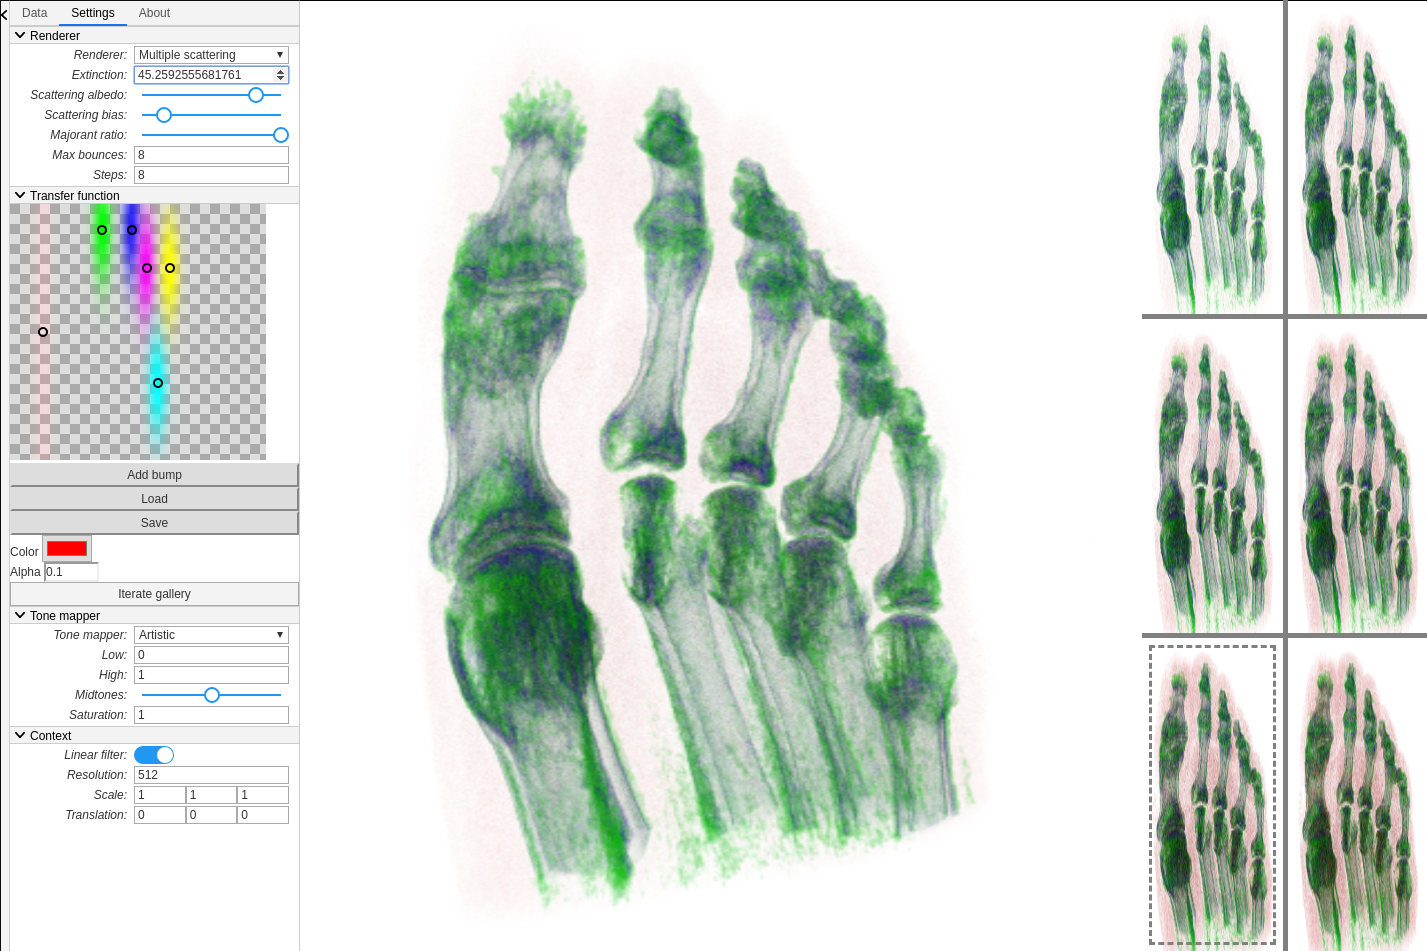
\includegraphics[width=.8\linewidth]{final_render.png}
   \caption{\label{fig:final}
    Final render, no manual adjustments of the transfer function}
\end{figure}

We chose to only use six bumps, which translates to six regions of the volume being recognized. With more bumps, the resulting image would be too cluttered and, depending on the dataset, some irrelevant parts of the volume could be recognized as important. 

An important feature of this approach is that the user can manually inspect and modify each of the generated transfer functions, at each iteration.  

The performance of the volume rendering procedure is slightly hindered, since multiple renders are being processed at the same time at the start of each iteration. The application still stays stable and usable in real-time, even on low performance hardware, such as a laptop with integrated graphics. 


\section{Conclusion}
Design gallery proves to be a good choice for semi-automatic transfer function creation, especially if the user is unfamiliar with the specific dataset he is trying to visualize. With the use of an iterative approach, we guide the user through the process of transfer function definition, providing the user with graphical feedback and manual adjusting at every step. 
The process could be enhanced by using a 2-dimensional histogram, in order to automatically detect the points in volume where the voxel gradients are the most pronounced. Additionally, more iterations could be added, where each of the parameters of each of the bumps could be set in a separate iteration. In order to better represent each of the materials in the volume, an opacity modulation could be used. 

%-------------------------------------------------------------------------

%\bibliographystyle{eg-alpha}
\bibliographystyle{eg-alpha-doi}

\bibliography{egbibsample}

%-------------------------------------------------------------------------


\end{document}

